\documentclass[sigconf]{acmart}

\usepackage{booktabs} % For formal tables
\usepackage{url}
\usepackage{graphicx}
\usepackage{subcaption}
\newcommand{\kai}[1]{{\bf \color{blue} [[Shukai says ``#1'']]}}
\newcommand{\heng}[1]{{\bf \color{cyan} [[Yuheng says ``#1'']]}}
\newcommand{\hao}[1]{{\bf \color{red} [[Hao says ``#1'']]}}
\newcommand{\hui}[1]{{\bf \color{purple} [[Zhenghui says ``#1'']]}}
% Copyright
%\setcopyright{none}
%\setcopyright{acmcopyright}
%\setcopyright{acmlicensed}
\setcopyright{rightsretained}
%\setcopyright{usgov}
%\setcopyright{usgovmixed}
%\setcopyright{cagov}
%\setcopyright{cagovmixed}


% DOI
%\acmDOI{10.475/123_4}

% ISBN
%\acmISBN{123-4567-24-567/08/06}

%Conference
\acmConference[CNW]{SJTU Computer Network Workshop}{December 2017}{Shanghai, China} 
\acmYear{2017}
\copyrightyear{2017}


%\acmArticle{4}
%\acmPrice{15.00}

% These commands are optional
%\acmBooktitle{Transactions of the ACM Woodstock conference}
%\editor{Jennifer B. Sartor}
%\editor{Theo D'Hondt}
%\editor{Wolfgang De Meuter}


\begin{document}
	\title{Predicting Internet Path Dynamics and Performance with Machine Learning}
	%\titlenote{Produces the permission block, and
	%  copyright information}
	%\subtitle{Extended Abstract}
	%\subtitlenote{The full version of the author's guide is available as
	%  \texttt{acmart.pdf} document}
	
	
	\author{Zhenghui Wang}
	\affiliation{%
		\institution{Shanghai Jiao Tong University}
		\city{Shanghai} 
		\state{China} 
		\postcode{200240}
	}
	\email{felixwzh@outlook.com}
	
	\author{Hao Wang}
	\affiliation{%
		\institution{Shanghai Jiao Tong University}
		\city{Shanghai} 
		\state{China} 
		\postcode{200240}
	}
	\email{?@?.com}
	
	\author{Yuheng Zhi}
	\affiliation{%
		\institution{Shanghai Jiao Tong University}
		\city{Shanghai} 
		\state{China} 
		\postcode{200240}
	}
	\email{?@?.com}
	
	\author{Shukai Liu}
	\affiliation{%
		\institution{Shanghai Jiao Tong University}
		\city{Shanghai} 
		\state{China} 
		\postcode{200240}
	}
	\email{?@?.com}
	
	% The default list of authors is too long for headers.
	\renewcommand{\shortauthors}{CN Group}
	
	
	\begin{abstract}
		We study the problem of predicting internet path dynamics and performance. We use \texttt{traceroute} measurement and machine learning models.
	\end{abstract}
	
	%
	% The code below should be generated by the tool at
	% http://dl.acm.org/ccs.cfm
	% Please copy and paste the code instead of the example below. 
	%
	\begin{CCSXML}
		<ccs2012>
		<concept>
		<concept_id>10010520.10010553.10010562</concept_id>
		<concept_desc>Computer systems organization~Embedded systems</concept_desc>
		<concept_significance>500</concept_significance>
		</concept>
		<concept>
		<concept_id>10010520.10010575.10010755</concept_id>
		<concept_desc>Computer systems organization~Redundancy</concept_desc>
		<concept_significance>300</concept_significance>
		</concept>
		<concept>
		<concept_id>10010520.10010553.10010554</concept_id>
		<concept_desc>Computer systems organization~Robotics</concept_desc>
		<concept_significance>100</concept_significance>
		</concept>
		<concept>
		<concept_id>10003033.10003083.10003095</concept_id>
		<concept_desc>Networks~Network reliability</concept_desc>
		<concept_significance>100</concept_significance>
		</concept>
		</ccs2012>  
	\end{CCSXML}
	
	%\ccsdesc[500]{Computer systems organization~Embedded systems}
	%\ccsdesc[300]{Computer systems organization~Redundancy}
	%\ccsdesc{Computer systems organization~Robotics}
	%\ccsdesc[100]{Networks~Network reliability}
	
	
	\keywords{TODO}
	
	
	\maketitle
	
	\hui{I think we should focus on the process not the final result, which is also important.}
	
	\section{Introduction}
	Internet paths change frequently due to inter/intra-domain routing changes, load balancing, and even misconfigurations and failures\cite{1}.
	%  V. Paxson. 1996. End-to-end Routing Behavior in the Internet. In Proceedings of the ACM SIGCOMM 1996 Conference (SIGCOMM ’96). ACM, New York, NY, USA.
	Some of these changes can seriously disrupt performance, causing longer round-trip times, congestion, or even loss of connectivity\cite{2}.
	%U. Javed, I. Cunha, D. Cho"nes, E. Katz-Bassett, T. Anderson, and A. Krishnamurthy. 2013. PoiRoot: Investigating the Root Cause of Interdomain Path Changes. In Proceedings of the ACM SIGCOMM 2013 Conference on SIGCOMM (SIGCOMM ’13). ACM, New York, NY, USA, 183–194.
	Thus, it is of great significant to predict Internet path dynamics and performance.
	
	In the original paper\cite{oripaper}, the authors focus on the problem of predicting Internet path changes and path performance using \texttt{traceroute} measurements. They use the recent route information of paths (route age for paths, route changes in the past, average RTT, etc) to do some predictions of paths. Their are three predict targets: $(i)$ the remaining life time of a route (i.e., the time before a route changes), $(ii)$ the number of route changes in a future timeslot, and $(iii)$ the average RTT  that the path $P$ will experience in the next \texttt{traceroute} measurement.
	
	To achieve these goals, they introduce a $NETPerfTrace$ system, which relies on a standard random forest model for prediction. Moreover, they use extensive evaluation on the impact of different input features by studying the correlations between the inputs and the prediction targets, as well as target selection techniques.
	
	The dataset the authors provide with is a full week of Paris- \texttt{traceroute} measurements performed through the M-Lab open
	Internet measurement initiative\footnote{https://www.measurementlab.net/}. They observe more than 450,000 different paths sampled through Paris-\texttt{traceroute} measurements from more than 180 geo-distributed servers. However, most of the paths are not periodically sampled during this week. And only 2,346 paths have at least 100 \texttt{traceroute} measurements during the analyzed week. So the dataset contains corresponding infomation of these 2,346 paths.
	
	We find some drawbacks in their data process.(see section \ref{sec:dataAna}) And in our own work, firstly we reprocess the provided data in more resonable ways and use the same method (random forest model) mentioned by the original paper\cite{oripaper} to compare the results. Secondly, another machine learning method, LSTM model, is applied to get better performance.
	
	\section{Related Works}
	In the original paper\cite{oripaper}, the problem they solve is to use random forest model to predict three targets for one path: $(i)$ the remaining life time of a route for one path at time $t$ (i.e., the time before a route changes), namely $R_r(t)$, $(ii)$ the number of route changes for one path $P$ in a future timeslot $T$, namely $rcP_T(t)$  and $(iii)$ the average RTT that the path $P$ will experience in the next \texttt{traceroute} measurement, namely $avgRTT_P(t)$.
	
	And to achieve these three targets, 69 input features are used to describe the statistical properties of route dynamics and path latency.
	
	For the first route dynamic target, the first group of 11 features,referred to as $F_A$, is chosen. It describes the statistical properties (average, minimum, maximum, and percentiles) of the route duration observed for each path.
	
	And for the second target, the second group of 14 features, as $F_B$, are relevant to the prediction of number of route changes. $F_B$ features take into account the statistical properties of route changes. In addition to that, $F_B$ contains information about the number of route changes observed for a path so far and a binary feature indicating whether a route change occurred for a path in the current time slot. 
	
	And the last group of 44 features ,referred to as $F_C$ decribes statistical properties of path latency, which is relavent to the prediction of the next \texttt{traceroute} measurement. They calculate the staistical properties of four RTT metrics (average, minimum, maximum and standard deviation) reported from each \texttt{traceroute} measurement.
	
	
	Then they study the correlation among the input features and the targets and apply  feature selection techniques to select the best features for prediction. When using as input the full set of 69 input features $F_A \cup F_B \cup F_C$, and perform wrapper-based feature selection on top of this full set. The result shows that the top important features for three targets are not necessarily the ones in corresponding $F_A,F_B$ or $F_C$.
	
	
	And the authors use three different ways of selecting input features: $(i)$  use all of the 69 features to predict each target, $(ii)$ when predicting target $X$, use corresponding feature set $F_X$, $(iii)$ after wrapper-based feature selection, use the top features for each target. And finally, what they get is the third way of choosing input features can achieve better results (though there is only minor difference in output results).
	
	
	\paragraph{Other Applications of MLCN}
	The last 2 decades has seen emerging applications of machine learning techniques used in computer networks \cite{kwon2017survey}. Classic methods, such as SVM, RBM, PCA and LDA, and deep learning methods including DBN, DNN and RNN, are both applied to areas like anomaly detection, web security, traffic prediction, etc. A usual procedure is to use autoencoders, both deep and classic ones, for dimensionality reduction and depend on SVM and DBN as a classifier.
	
	Here we mention a few representative works. Alom et al. \cite{alom2015intrusion} focus on intrusion detection system. Tao et al. \cite{tao2016big} search to build a data fusion algorithm with awareness of network security situation obtained by PCA, LDA and Fisher score. Lv et al. \cite{lv2015traffic} first develop deep learning methods in traffic flow prediction. Hou et al. \cite{hou2010malicious} aims to learn filtering rules for malicious contents automatically. Thottan et al.~\cite{thottan2003anomaly} are among the first to introduce self-learning methods to anomaly detection and a series of botnet detection methods follows up \cite{ranjan2014machine, singh2014big, beigi2014towards, zhao2013botnet}.
	
	\paragraph{Random Forest} Random Forest is a classical model in machine learning. It basically integrates a bunch of decision trees trained on different parts of the dataset, thus eliminating the risk of overfitting when a single tree is trained. A Random Forest makes predictions by averaging that of all the decision trees in it or by taking the majority vote in classification scenario. In addition, recent years have seen the development of Deep Random Forest, which employs the superior descriptive ability of deep models in the prediction process as well as maintaining the explanatory of decision tree-based models.
	
	\paragraph{LSTM} LSTM is an improved version of the original RNN, which largely resolved the problem of gradient vanishing and explosion in original RNN and is capable of capturing multi-scale dependencies in sequential data. The main modification it made to the original RNN unit is to add multiplicative \textbf{gate} unit that control the proportions of information to forget/pass on to the next time step. Even more modern version of LSTM like BLSTM equip the model with the ability to learn from the future, but here we only use the basic LSTM to explore the time dependencies in the dataset.
	
	\section{Data Analysis}
	\label{sec:dataAna}
	\hui{I think this is an important part, who will take this part?}
	\heng{Plots of temporally differentiated prediction targets are given here to show their behavior patterns in temporal domain, thus supporting the use of LSTMs.}
	With careful review of the data used in the original paper, here we: $(i)$ show the authors had used the data incorrectly in the context of making predictions, and $(ii)$ reveal the temporal properties that the original method failed to employ but perfectly fits LSTM model (long short term memory neural networks), which we will later use to improve the performance.
	\subsection{Justification of Data Processing}
	The original paper \cite{oripaper} made a major mistake on data employment: they implicitly used data from the future to predict events in the future, which is not possible. More specifically, all of their tests on the performance of \textit{NetPerfTrace} depend on statistics calculated out of data of all time, including the data they were to predict. Features like percentiles of route life, for example, take the route life of all routes during the whole week into account, including route $r_i$. However, these features still take part in predicting the residual life of $r_i$. It resembles guessing something you already knew.
	
	In fact, a principle of making predictions is to use the data already observed to guess the unobserved. Thus, in all the experiments of this paper, we made it a hard constraint that all the features used to predict any event at, say, time $t$, only come from the raw data collected before $t$. First, we re-validated the performance of classic machine learning method on two tasks(task 1 and task 3) according to our justified data processing manner, (The reason why we miss the task 2 is that it is not possible to reprocess data with respect to task 2 according to the raw data given by the original paper) in the following three ways: $(i)$ use the global statistical features (average, minimum, maximum, and percentiles, etc) of the former $k\%$ data to train the models and predict the targets of the latter $(1-k)\%$ data, $(ii)$ use the global features to train the models and update them during the predicting procedure and $(iii)$ use data in a certain recent time-slot to calculate the global features. Then we train LSTMs on these data in two different ways: $(i)$ input only a scalar, the prediction target, to the network and $(ii)$ input the prediction target and the global features as a vector.
	
	\subsection{Temporal Properties of the Data}
	We believe temporally adjacent routes and \texttt{traceroute} records of a path share some common network nodes, thus their behavior contain implicit dependencies in temporal domain. While the data are organized in the order of time, the original method ignored this property but regard them as independent instances, i.e., the prediction for the next time step only depends on the features of the present, but does not use information given by more previous time steps. This manner fails the original method to capture even the most naive temporal dependencies. Here we do not provide strict proofs of the temporal dependencies that lie in these routes but simply throw some light on the possibility of their existence.
	\begin{figure*} 	
		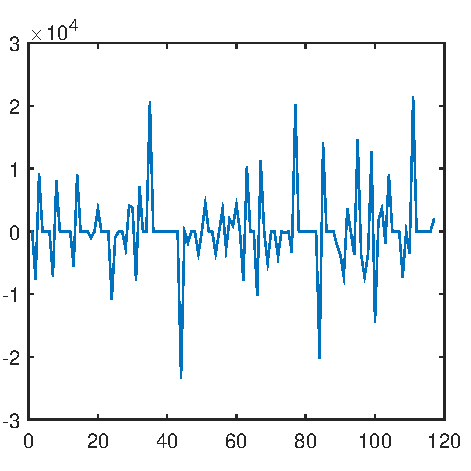
\includegraphics[width=0.22\textwidth]{fig/total_life_8} 
		\label{fig:3.1a}
		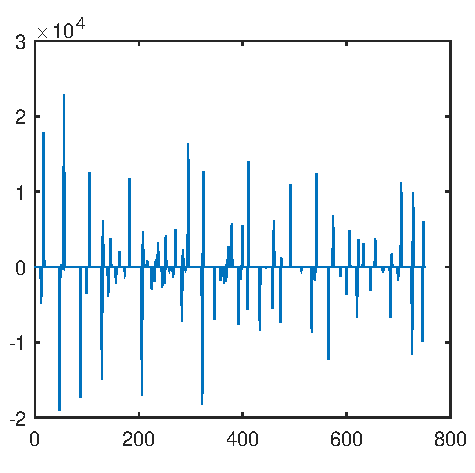
\includegraphics[width=0.22\textwidth]{fig/total_life_20}
		\label{fig:3.1b}
		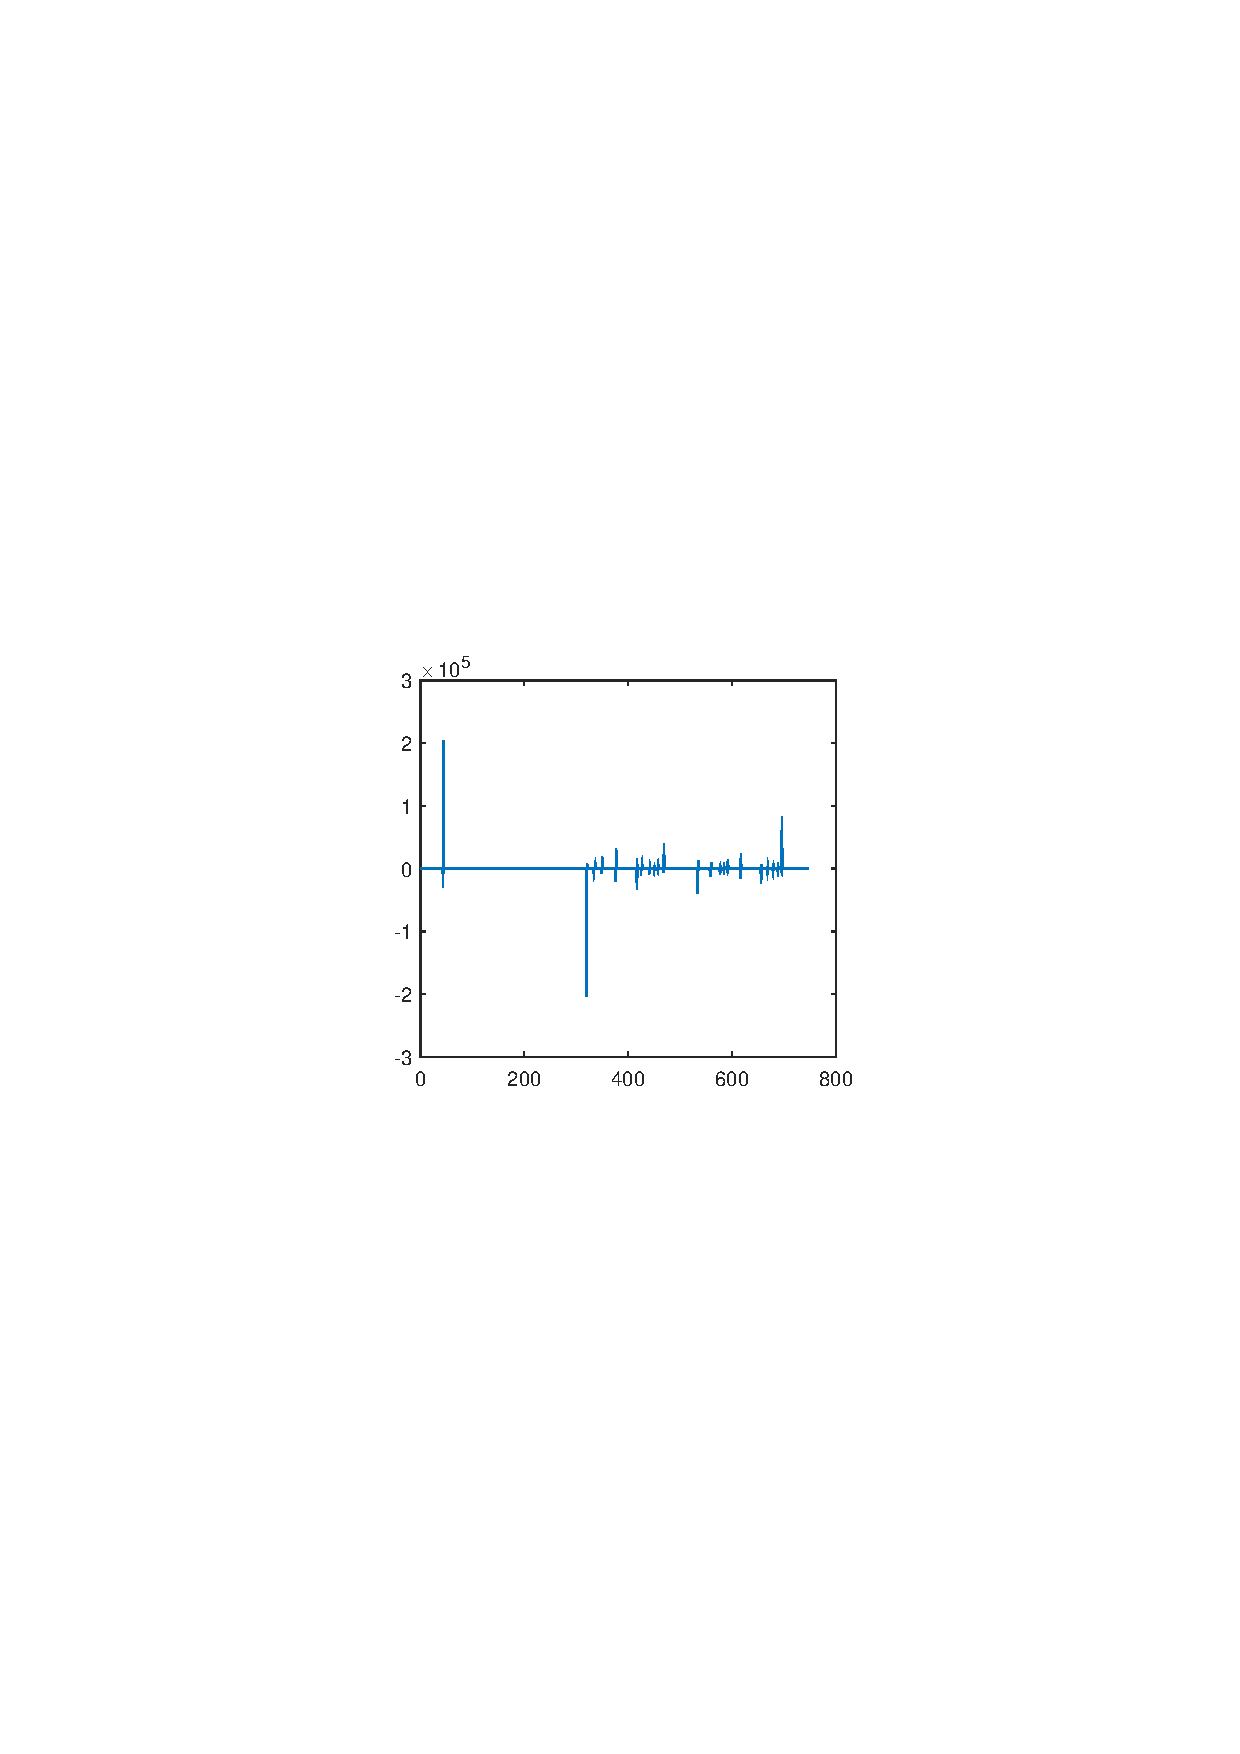
\includegraphics[width=0.22\textwidth]{fig/total_life_21}
		\label{fig:3.1c}
		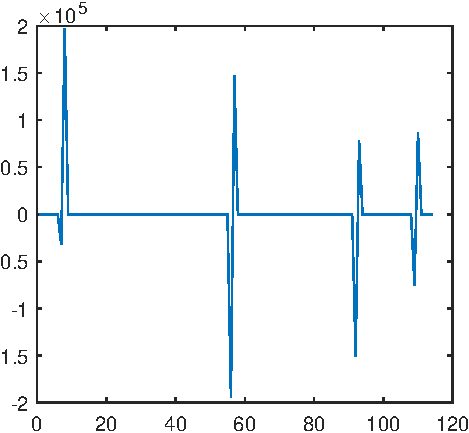
\includegraphics[width=0.22\textwidth]{fig/total_life_30}
		\label{fig:3.1d}

		%\vspace{-20pt}  
		\caption{Temporal patterns of route life among 4 different paths.}
		\label{fig:3.1}  
		%\vspace{-10pt}  
	\end{figure*}

\begin{figure*} 	
	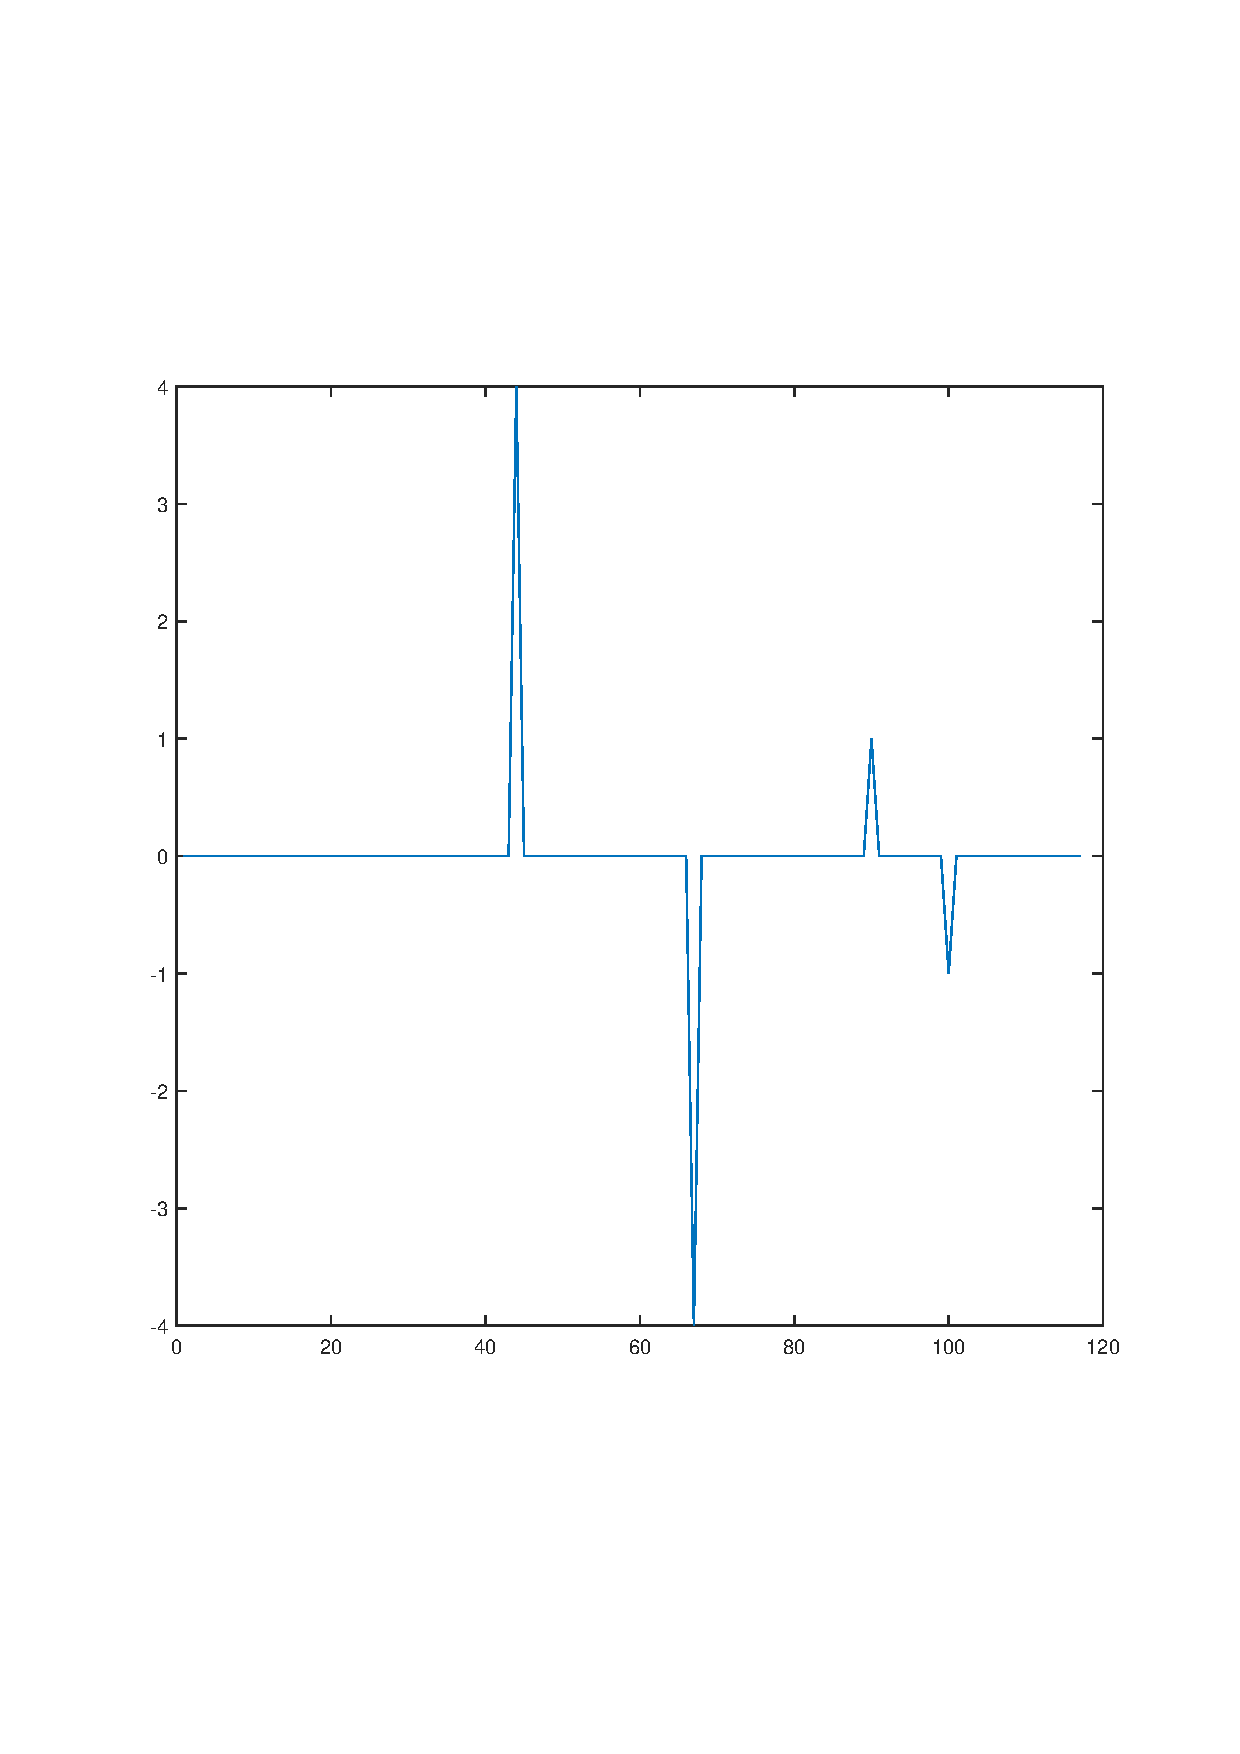
\includegraphics[width=0.22\textwidth]{fig/route_change_8} 
	\label{fig:3.2a}
	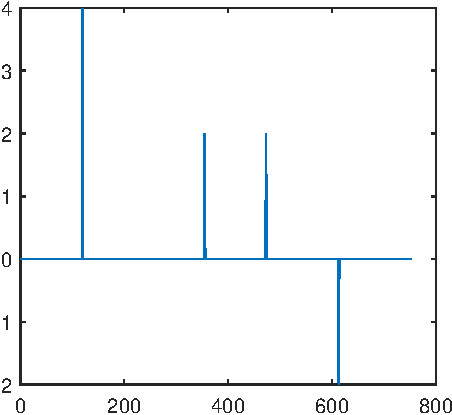
\includegraphics[width=0.22\textwidth]{fig/route_change_20}
	\label{fig:3.2b}
	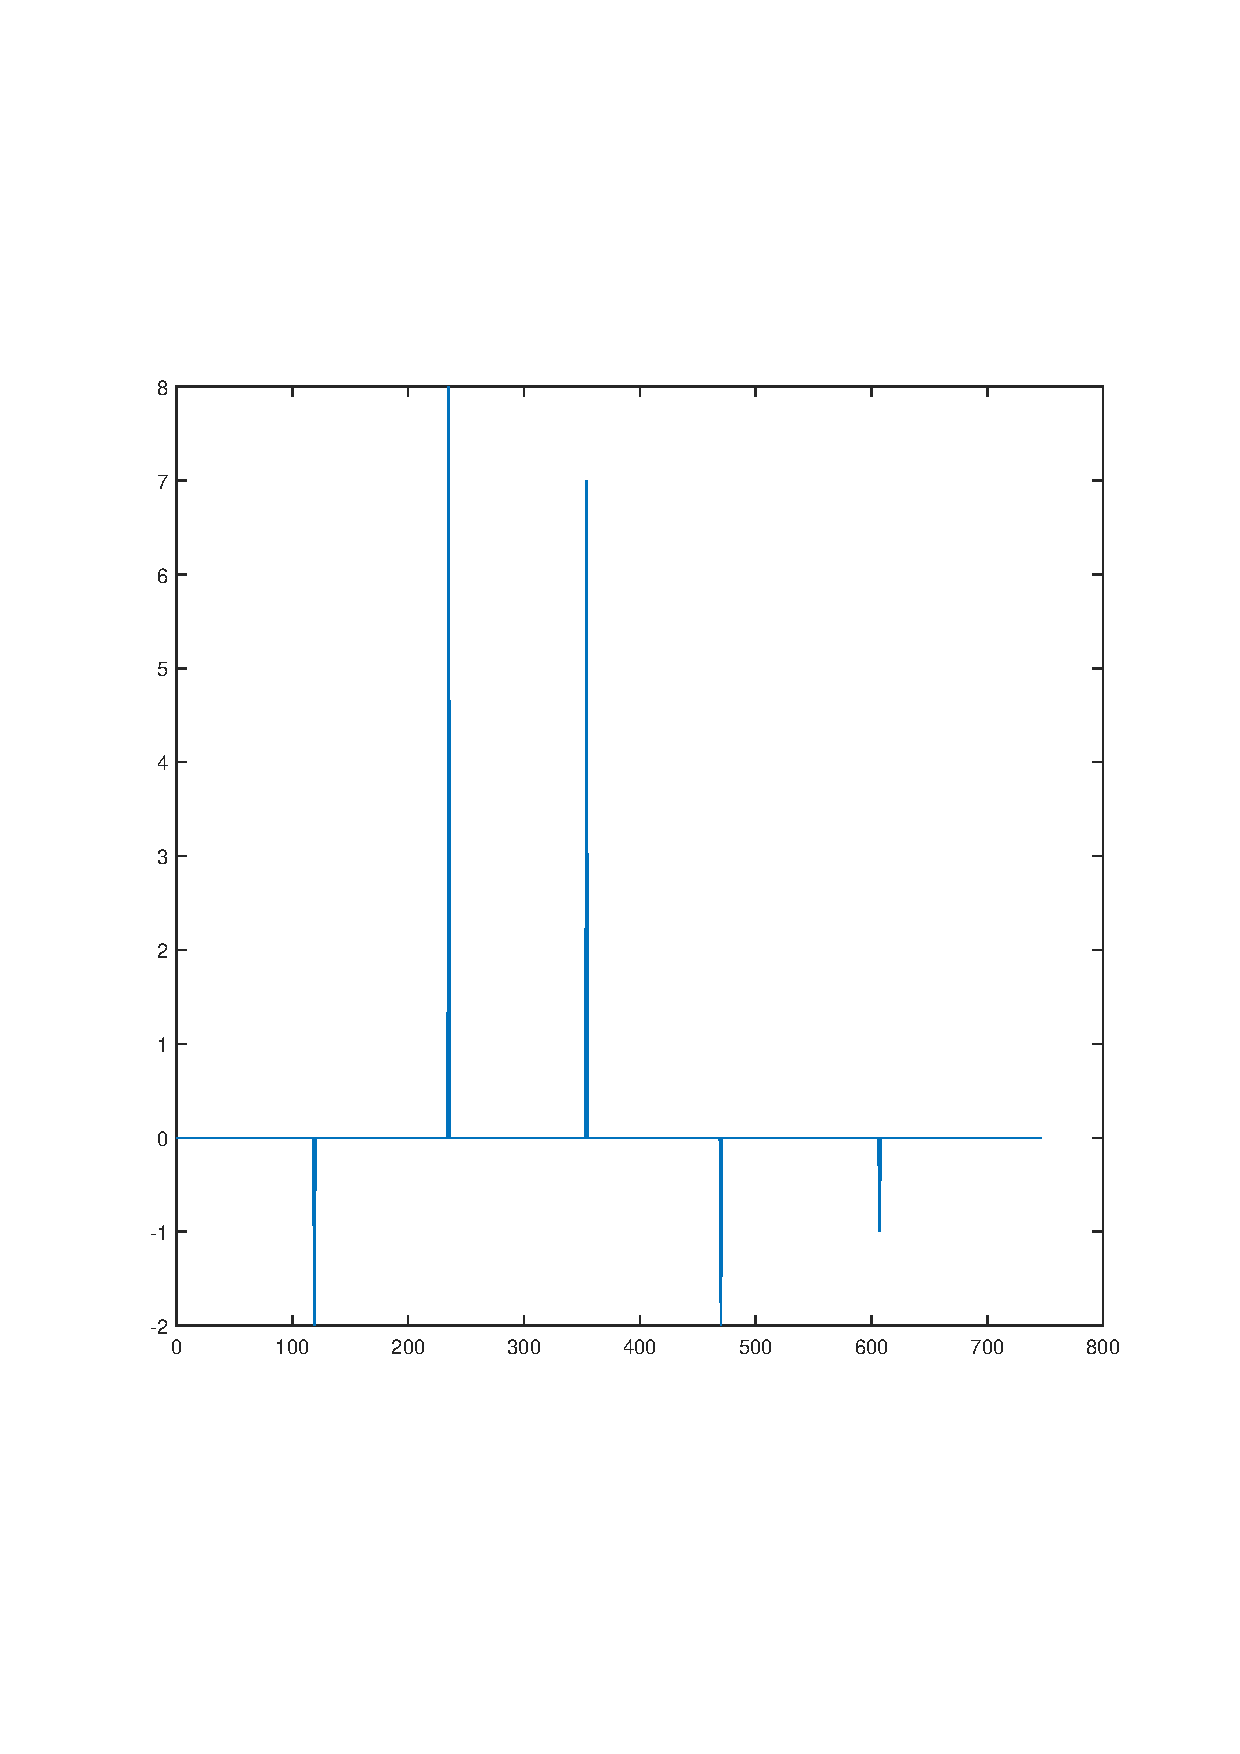
\includegraphics[width=0.22\textwidth]{fig/route_change_21}
	\label{fig:3.2c}
	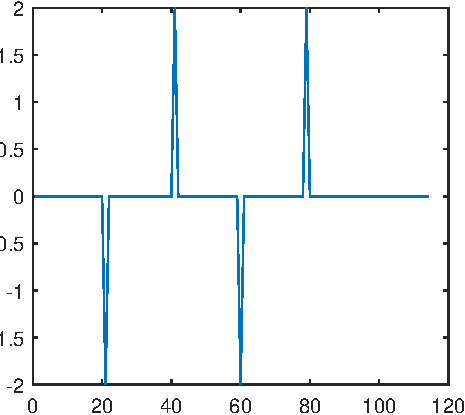
\includegraphics[width=0.22\textwidth]{fig/route_change_30}
	\label{fig:3.2d}
	
	%\vspace{-20pt}  
	\caption{Temporal patterns of the number of route changes among 4 different paths.}
	\label{fig:3.2}  
	%\vspace{-10pt}  
\end{figure*}

\begin{figure*} 	
	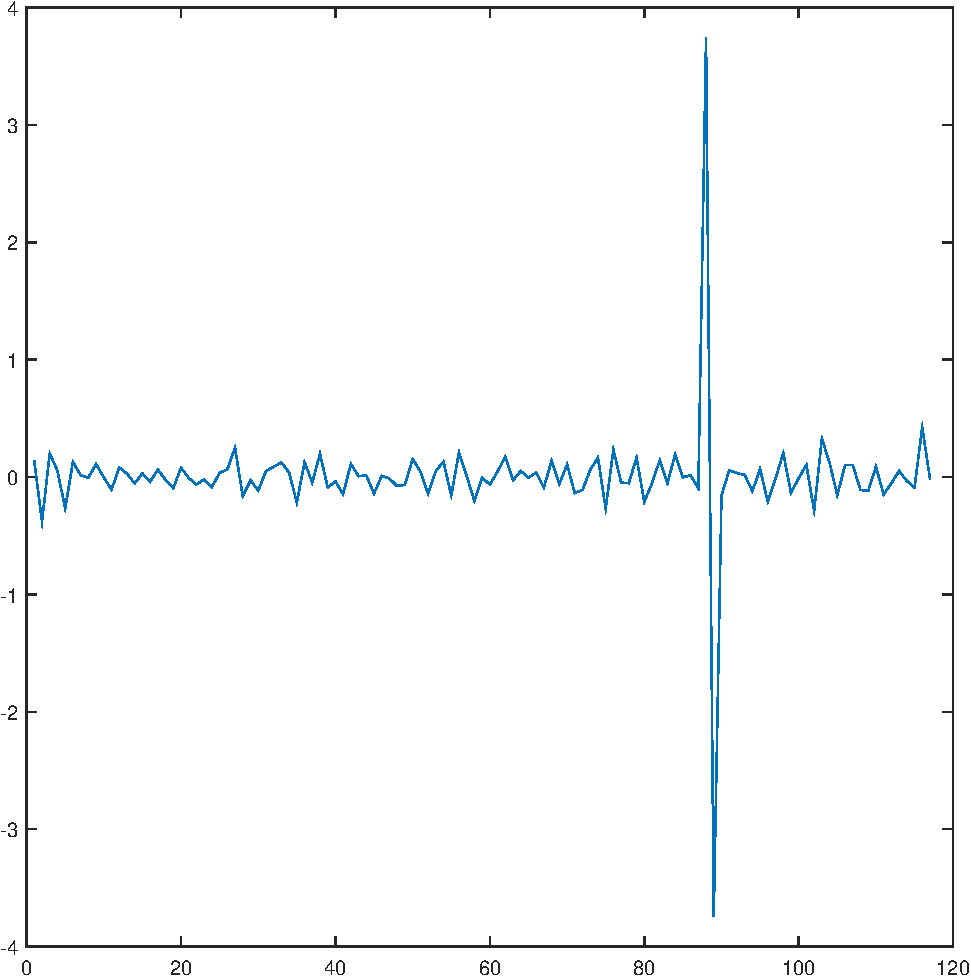
\includegraphics[width=0.22\textwidth]{fig/RTT_8} 
	\label{fig:3.3a}
	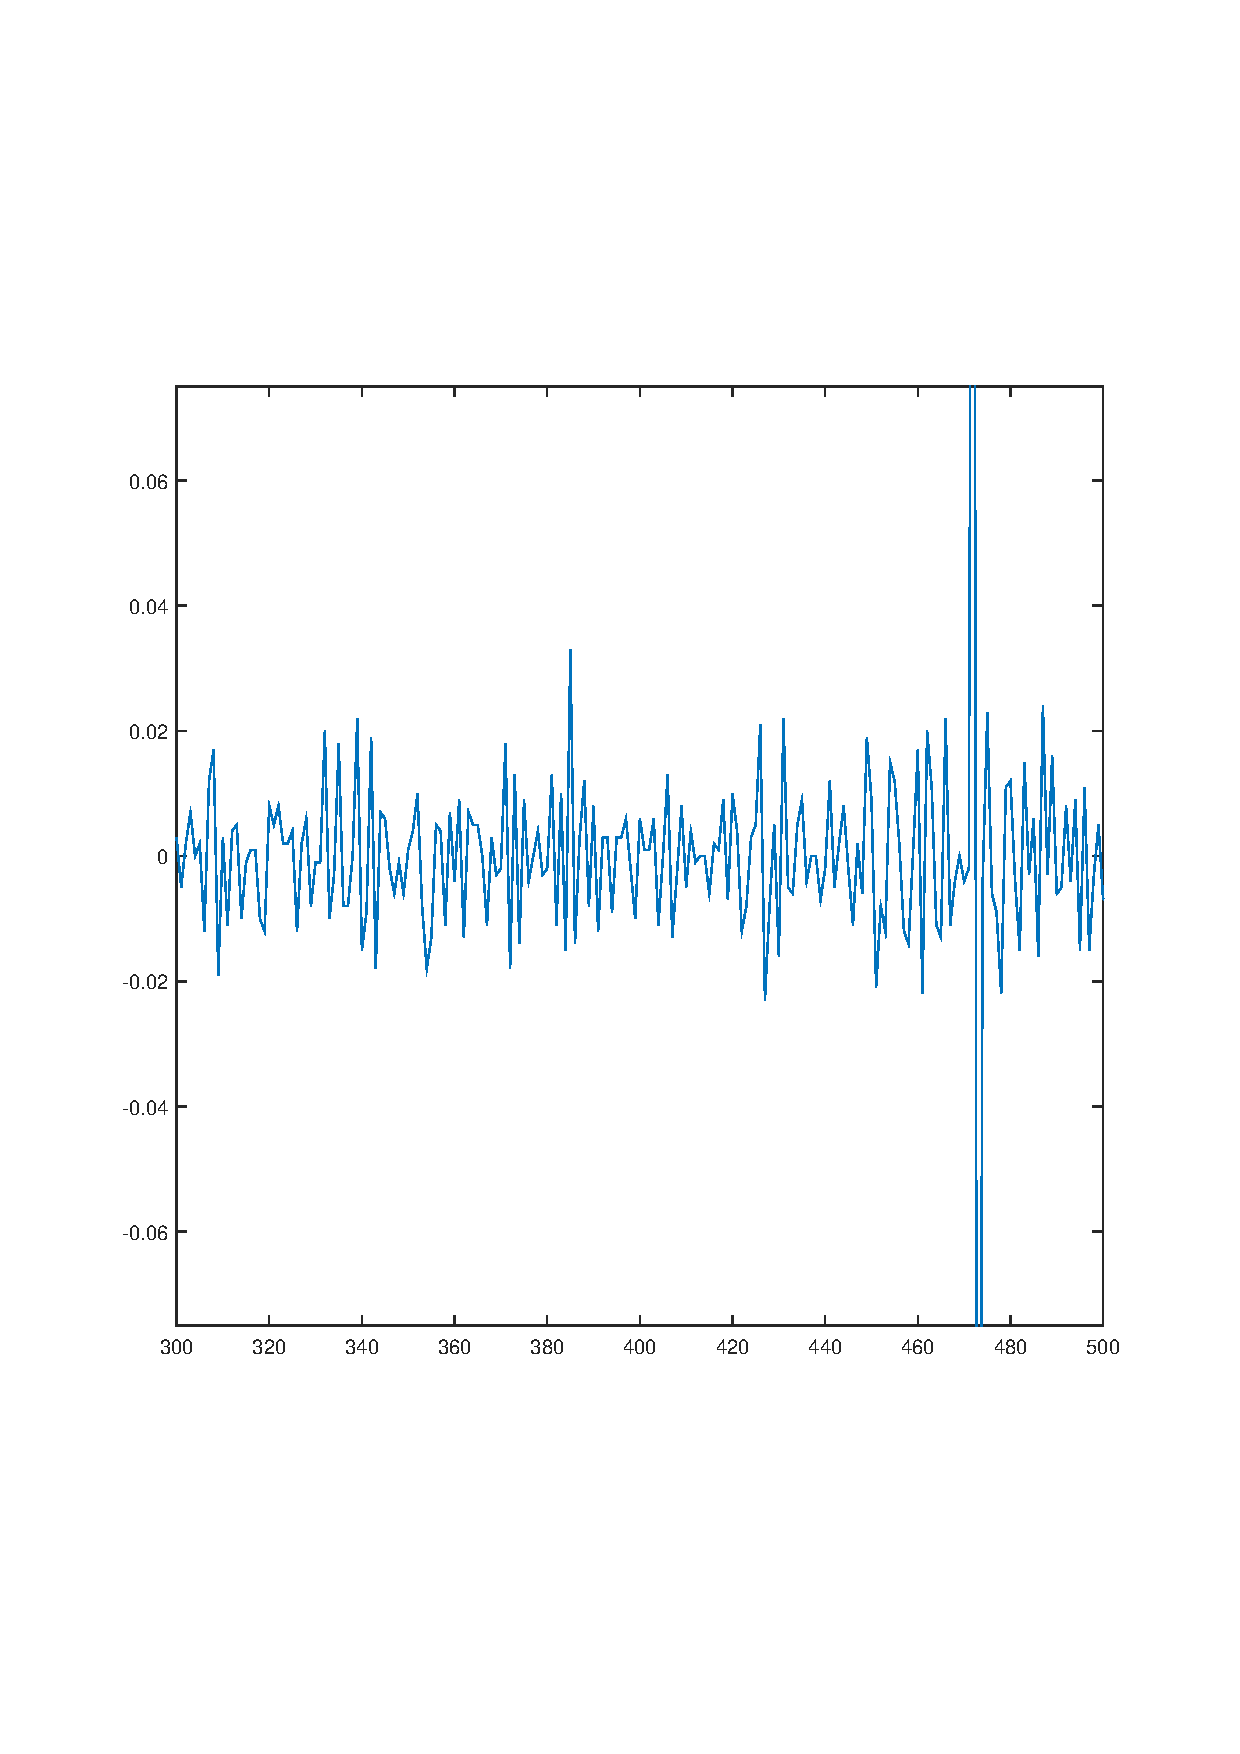
\includegraphics[width=0.22\textwidth]{fig/RTT_20}
	\label{fig:3.3b}
	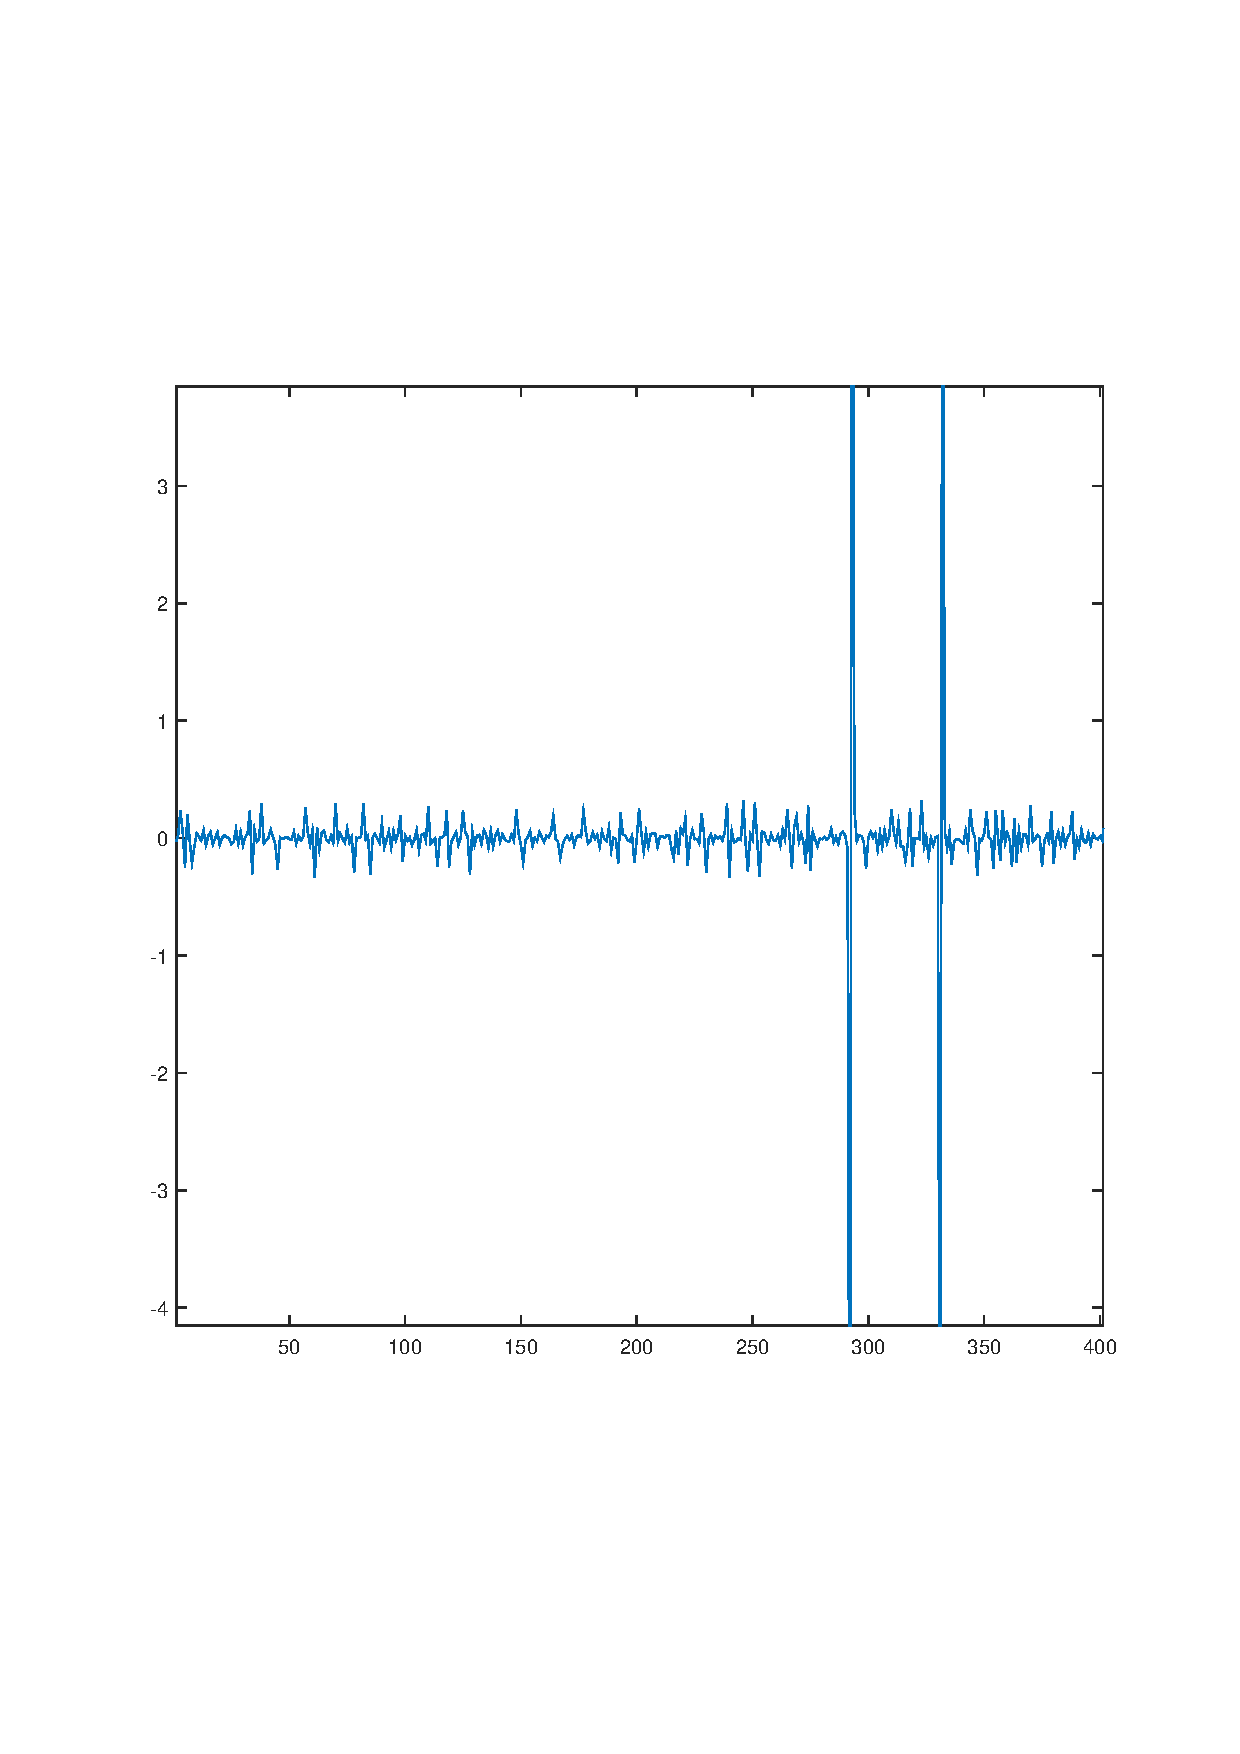
\includegraphics[width=0.22\textwidth]{fig/RTT_21}
	\label{fig:3.3c}
	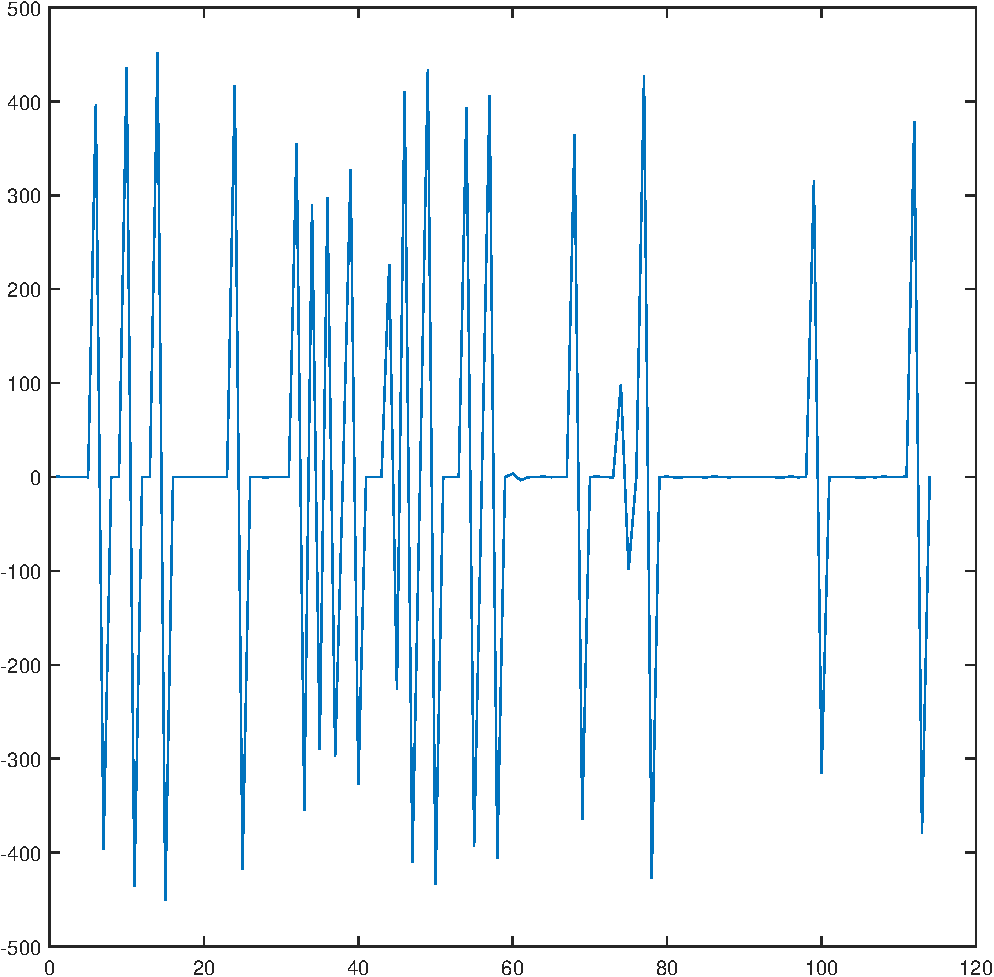
\includegraphics[width=0.22\textwidth]{fig/RTT_30}
	\label{fig:3.3d}
	
	%\vspace{-20pt}  
	\caption{Temporal patterns of round trip time among 4 different paths.}
	\label{fig:3.3}  
	%\vspace{-10pt}  
\end{figure*}
	
	Applying simple differential analysis to the raw data, we found the prediction targets indeed show local temporal patterns which we can hopefully capture with LSTMs. \textbf{Fig.\ref{fig:3.1}}, \textbf{Fig.\ref{fig:3.2}} and \textbf{Fig.\ref{fig:3.3}} exhibit differentiated results of the three prediction targets in different paths. We can see that these paths behave in somehow consistent temporal patterns along their own ways but differently from each other.
	
	No more solid evidence could be provided to prove the periodicity of these patterns because pattern itself is hard to define. However, these results are already enough to make us hopeful about the performance of LSTMs, which are expert in capturing temporal dependencies, no-matter long-term ones or short-term ones.
	
	\section{Methodology}
	\subsection{Data Processing}
	We reprocess the data in several more rational ways, which in other words, predicting targets using the previous \texttt{traceroute} data only. And to be specific, we divide the data into two sets, namely training set and test set. We calculate statistical properties (global features) of paths using three different manners: $(i)$ use the global features (max, min, average, percentiles, etc.) in the training set to get the model and predict the targets of the latter $(1-k)\%$ data, $(ii)$ use the global feature of the former $k\%$ to train the models and update these features during the predicting procedure(i.e.,update the global features everytime there is a new \texttt{traceroute} measurement of a path), and $(iii)$ only use recent \texttt{traceroute} data of certain length (namely $window\ size$) in the training set to calculate the global features, and when using the trained model to predict targets, we only consider features calculated in  recent \texttt{traceroute} measurements of the same $window\ size$ . For convenience, in the following article, we use $data-i$ to represent reprocessing the original data using the $i$th processing manner ($i$ can be either 1,2 or 3). And for the third processing manner, we use $data-3-ws\#$ to indicate the $window\ size$ of $\#$.
	
	\subsection{LSTM Model}
	In order to leverage the prediction targets' character of temporal locality, we further use LSTM to do time series modeling. More formally, we take $t-1$ most recent \texttt{traceroute} measurements features $(\mathbf{x_1},\mathbf{x_2},...,\mathbf{x_{t-2}},\mathbf{x_{t-1}})$and the current \texttt{traceroute} measurement feature $\mathbf{x_t}$ together as the input, i.e., $\mathbf{X}=(\mathbf{x_1}, \mathbf{x_2},...,\mathbf{x_{t-1}}, \mathbf{x_{t}})$ And the out put is a single scalar $\hat{y}$ which is supposed to be the prediction of the target $y$.
	Let $G_{\theta}(\mathbf{x_i},\mathbf{h_i})$ the $\theta$ parameterized LSTM, we have:
	\begin{equation}
	\mathbf{h_{i+1}}=G_{\theta}(\mathbf{x_i},\mathbf{h_i}),
	\end{equation}iteratively. and when we have the $\mathbf{h_{t}}$, we calculate our final prediction $\hat{y}$ by a fully connected layer with parameter $\mathbf{W}$:
	\begin{equation}
	\hat{y}=\mathbf{W}\cdot\mathbf{h_t},
	\end{equation}
	and the loss function is:
	\begin{equation}
	\mathcal{L}=\frac{1}{n}\sum_{i=1}^{n}(y_i-\hat{y_i})^2.
	\end{equation}
	The training objective is to minimize $\mathcal{L}$.
	
	
	
	\section{Experiment}
	\subsection{Random Forest Model}
	In our experiment, firstly, we use the standard random forest model (the same as the original paper) with the reprocessed data.  In practice, we set $k = 70, 80$ respectively. And in the third processing manner, the $window\ size$ is set to $10,20$ and $50$ recent \texttt{traceroute} measurements, respectively. We find that there is little difference when setting $k$ either to 70 or 80. Below are the results when $k = 70$. And we also define an evaluation metric $ABC$, which indicates the  area below the curve ($ABC\in[0,1]$). The closer $ABC$ is to $1$, the better prediction result it has. These figures in \textbf{Fig.\ref{fig:task1_RF}} and \textbf{Fig.\ref{fig:task3_RF}} illustrate the relationship between sample percentage and relative prediction error(i.e., $\mid Real - Predict\mid/ Real $). 
	\begin{figure*} [!htb] 
		%\vspace{-4pt}  
		\centering  
		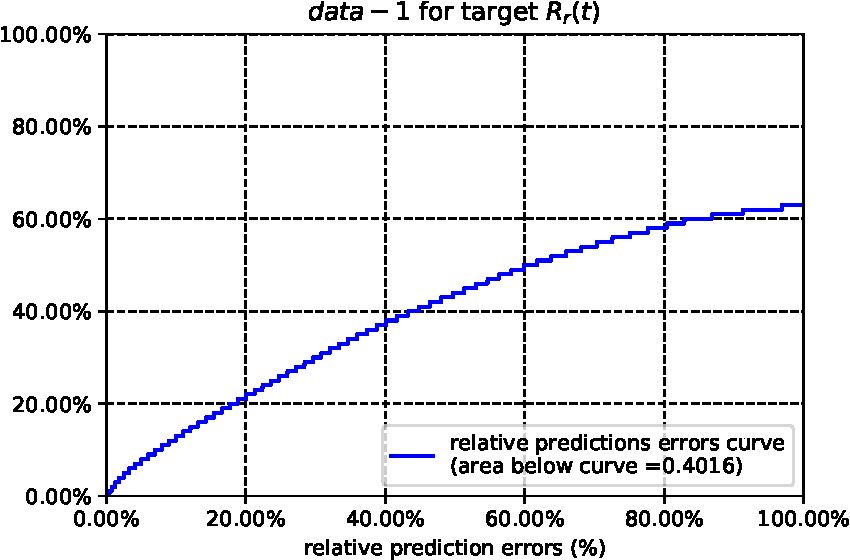
\includegraphics[width=0.3\textwidth]{fig4/data-1-task-1-7030-RF.pdf}  
		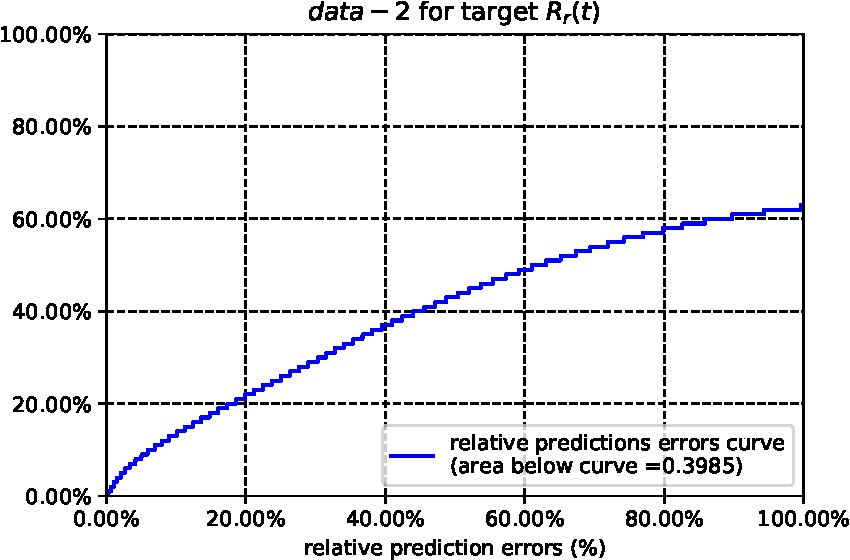
\includegraphics[width=0.3\textwidth]{fig4/data-2-task-1-7030-RF.pdf} 
	\end{figure*} 
	\begin{figure*} 	
		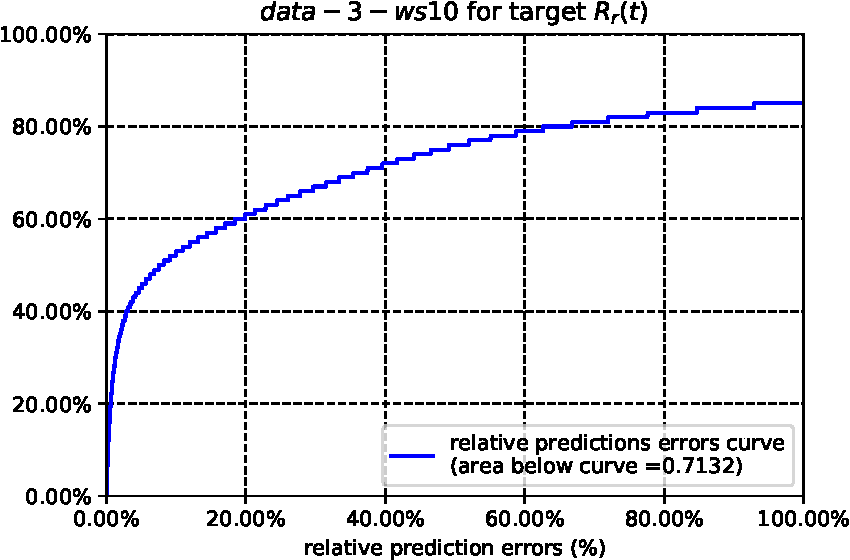
\includegraphics[width=0.3\textwidth]{fig4/data-3-task-1-7030-windowsize10-RF.pdf} 
		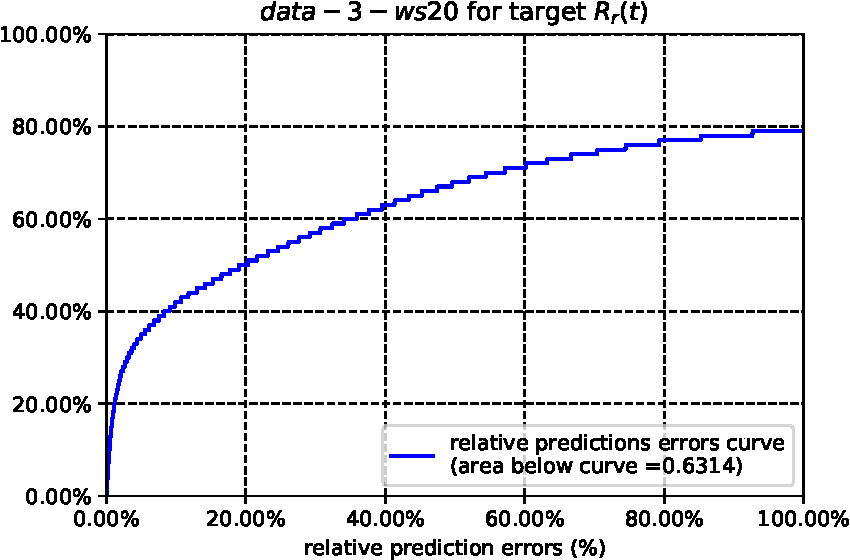
\includegraphics[width=0.3\textwidth]{fig4/data-3-task-1-7030-windowsize20-RF.pdf}
		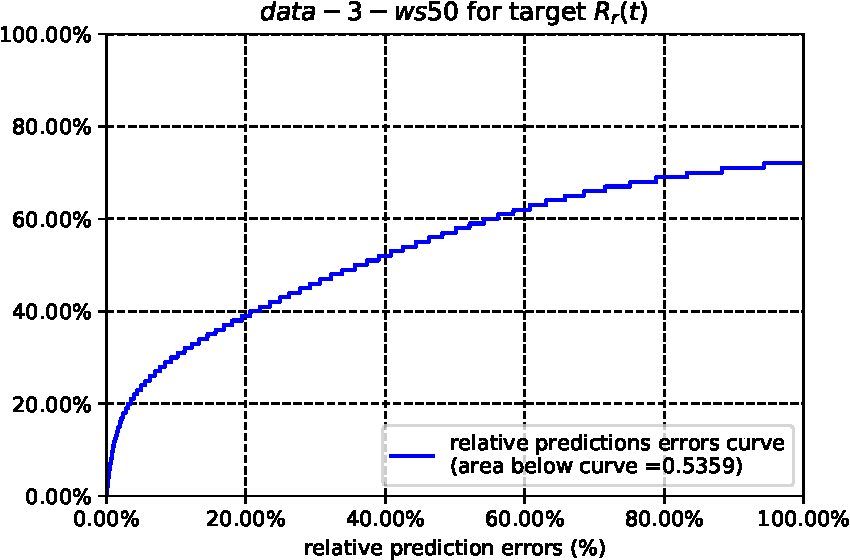
\includegraphics[width=0.3\textwidth]{fig4/data-3-task-1-7030-windowsize50-RF.pdf}
		%\vspace{-20pt}  
		\caption{Relative prediction errors for $R_r(t)$ of random forest models.}
		\label{fig:task1_RF}  
		%\vspace{-10pt}  
	\end{figure*}
	
	\begin{figure*} [!htb] 
		%\vspace{-4pt}  
		\centering  
		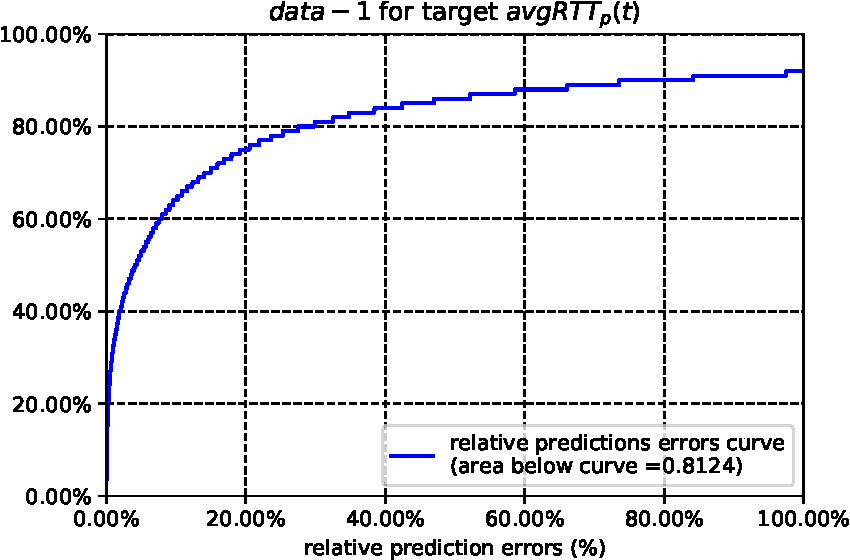
\includegraphics[width=0.3\textwidth]{fig4/data-1-task-3-7030-RF.pdf}  
		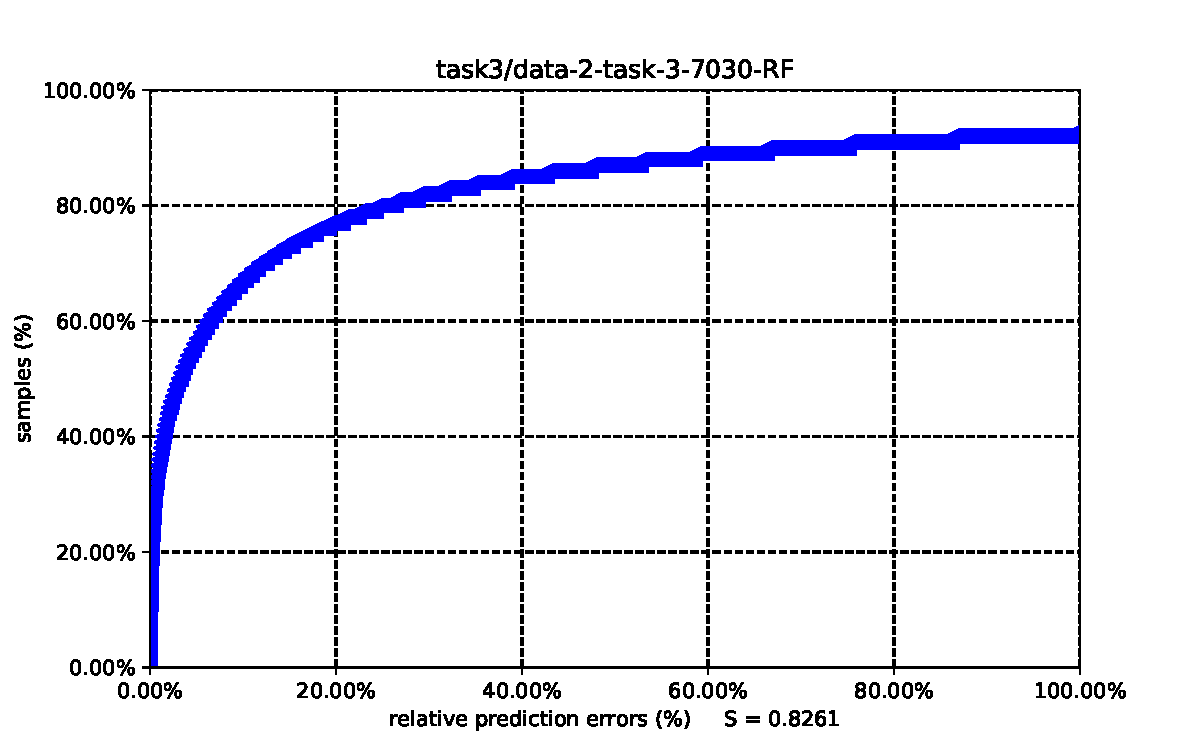
\includegraphics[width=0.3\textwidth]{fig4/data-2-task-3-7030-RF.pdf} 
	\end{figure*} 
	\begin{figure*} 	
		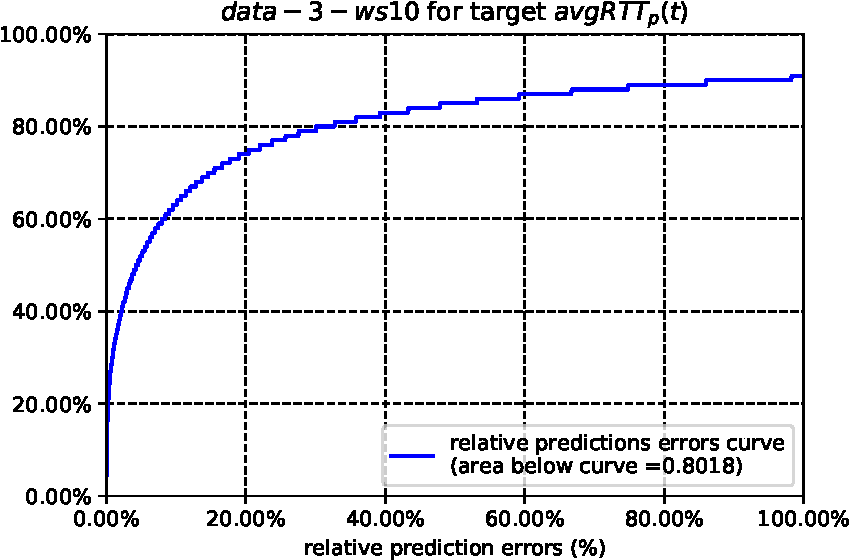
\includegraphics[width=0.3\textwidth]{fig4/data-3-task-3-7030-windowsize10-RF.pdf}
		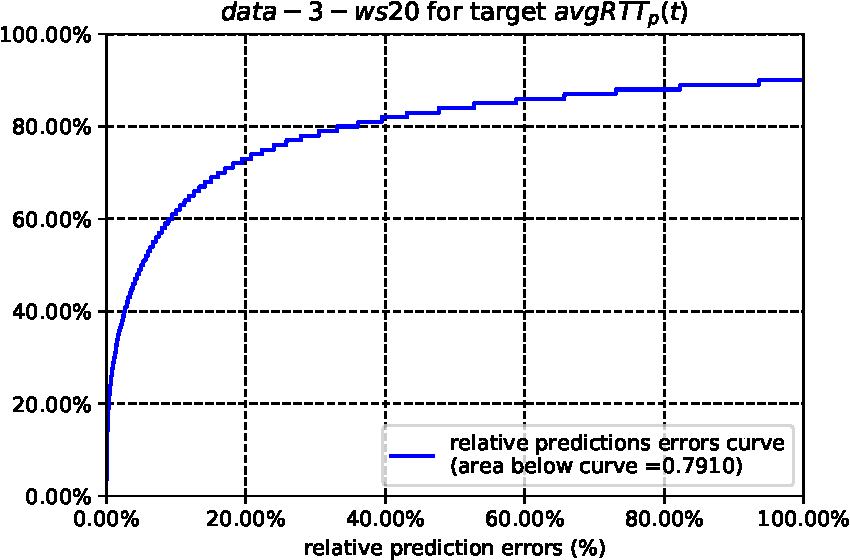
\includegraphics[width=0.3\textwidth]{fig4/data-3-task-3-7030-windowsize20-RF.pdf}
		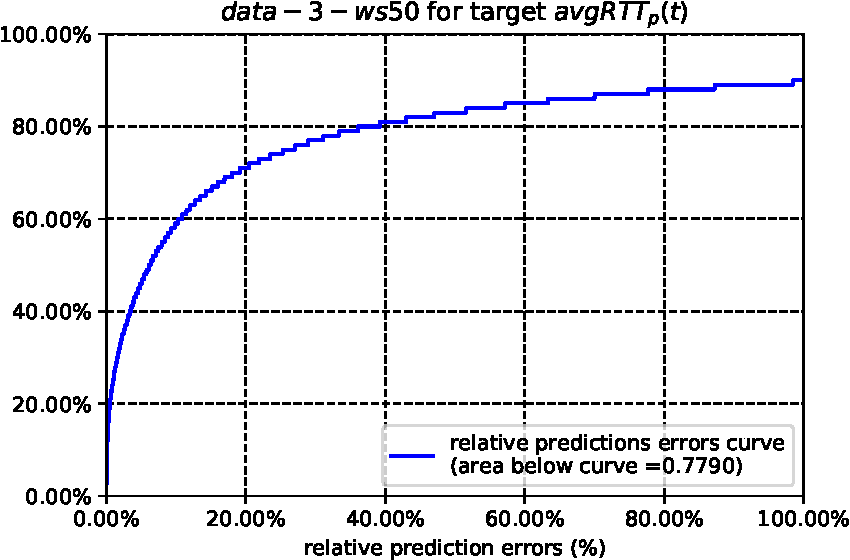
\includegraphics[width=0.3\textwidth]{fig4/data-3-task-3-7030-windowsize50-RF.pdf}
		%\vspace{-20pt}  
		\caption{Relative prediction errors for $avgRTT_P(t)$ of random forest models.}
		\label{fig:task3_RF}
		%\vspace{-10pt}  
	\end{figure*}
	
	\textbf{Tab.\ref{tab:result_RF}} describes the $ABC$ of two tasks in different data processing manner.
	\begin{table}[tbp]
		\centering  
		\begin{tabular}{lcc} 
			\hline
			Target &$R_r(t)$ &$avgRTT_P(t)$ \\ \hline
			\textit{data-1} & 0.4016    &0.8124   \\        
			\textit{data-2} &0.3985 &0.8261 \\        
			\textit{data-3-ws10}  &0.7132 &0.8018 \\
			\textit{data-3-ws20} &0.6314 &0.7910 \\
			\textit{data-3-ws50} &0.5359  &0.7790 \\ \hline
		\end{tabular}
		\caption{Experiment results($ABC$) of random forest models. }
		\label{tab:result_RF}
	\end{table}
	From \textbf{Tab.\ref{tab:result_RF}}, it can be inferred that for target $avgRTT_P(t)$: there is minor difference in processing the data in different manners . They all achieve relatively good results, which also indicates that for average RTT reported from \texttt{traceroute} measurement, it is not sensitive to the temporal locality. However, for the first predicting target, $R_r(t)$, it is very sensitive to the temporal locality. It changes rapidly as time changes. And to achieve better prediction result, using too much previous data will result in noise and decrease the performance of the model. Because from \textbf{Tab.\ref{tab:result_RF}}, we can clearly observe that $data-3-ws10$ achieves the largest $ABC$ compared with other processing manners. It considers only the recent data in a relatively short time slot. Indeed, it is reasonable to get such conclusion, for the remaining life time of a route is always closely related to their route age (which can be indicated from the recent previous \texttt{traceroute} data).
	\subsection{LSTM Model}
	
	As we observed above, among the 3 different \textit{window size} (10, 20, 50), \textit{window size} of 10 has the best performance. Thus, we set the timesteps for our LSTM model to be 10, either.  We adopt two kinds of input for the LSTM at each timestep: $(i)$ scalar and $(ii)$ vector.
	
	\begin{figure*} 	
		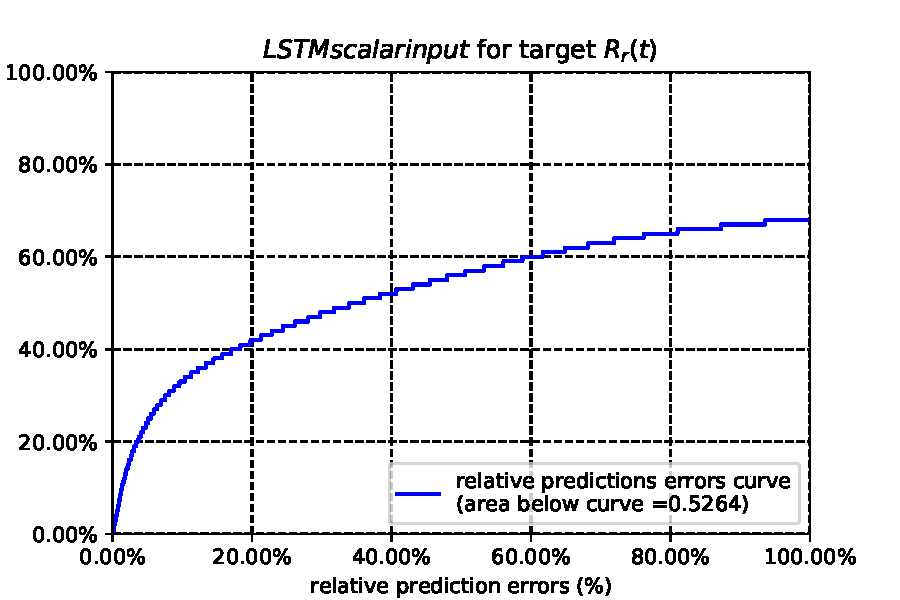
\includegraphics[width=0.3\textwidth]{fig4/task1-scalar-lstm.pdf}
		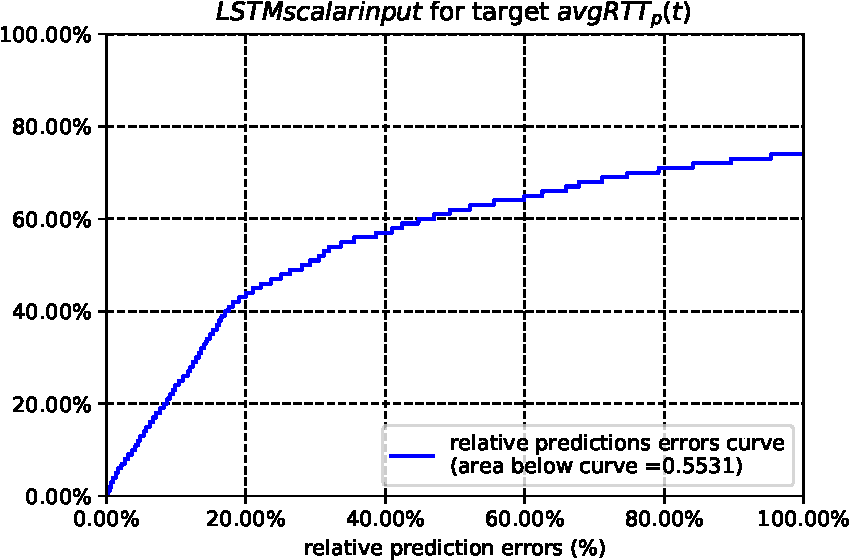
\includegraphics[width=0.3\textwidth]{fig4/task3-scalar-lstm.pdf}
		%\vspace{-20pt}  
		\caption{Relative prediction errors for $R_r(t)$ and $avgRTT_P(t)$ of LSTM models with scalar input.}
		\label{fig:lstm_scalar}
		%\vspace{-10pt}  
	\end{figure*}
	
	
	\subsubsection{Scalar Input}
	\begin{table}[t]
		\centering
		\begin{tabular}{lcc}
			\toprule
			{Target} &{$R_r(t)$} &{$avgRTT_P(t)$}\\
			\midrule
			\textit{LSTM-scalar-input} & 0.5264& 0.5530  \\
			\bottomrule
		\end{tabular}
		\caption{ Experiment results($ABC$) of LSTM models with scalar input. }
		\label{tab:lstm-scalar}
	\end{table}
	
	
	Since we have observed some local temporal patterns with the prediction targets, The most naive approach is to feed LSTM with the previous observed scalar without any statistics of it. \textbf{Fig.\ref{fig:lstm_scalar}} and \textbf{Tab.\ref{tab:lstm-scalar}} show the results.
	
	As we can see, for target $R_r(t)$, the $ABC$ of LSTM is larger	 than random forest with \textit{data-1} and \textit{data-2}, but is much smaller than random forest with \textit{data-3-ws10}. This shows empirical evidence that there is temporal locality with $R_r(t)$ of a path. We can infer $R_r(t)$ of a path from its recent \texttt{traceroute} measurements better than using current features only.
	
	By contrast, for target $avgRTT_P(t)$, the $ABC$ of LSTM is smaller than random forest in all cases, which may indicate that $avgRTT_P(t)$ is less likely to have the temporal locality.
	
	For both tasks, using scalar input for LSTM cannot outperform random forest steadily.
	
	\subsubsection{Vector Input}
	In order to better leverage the data to get better performance with our LSTM model, we take the same featues for LSTM model as those for random forest model. More specifically, Features for target $R_r(t)$ and Features for target $avgRTT_P(t)$.The results are shown in \textbf{Fig.\ref{fig:lstm-task1-vector}}, \textbf{Fig.\ref{fig:lstm-task3-vector}} and \textbf{Tab.\ref{tab:lstm-vector}}.
	
	\begin{figure*} 	
		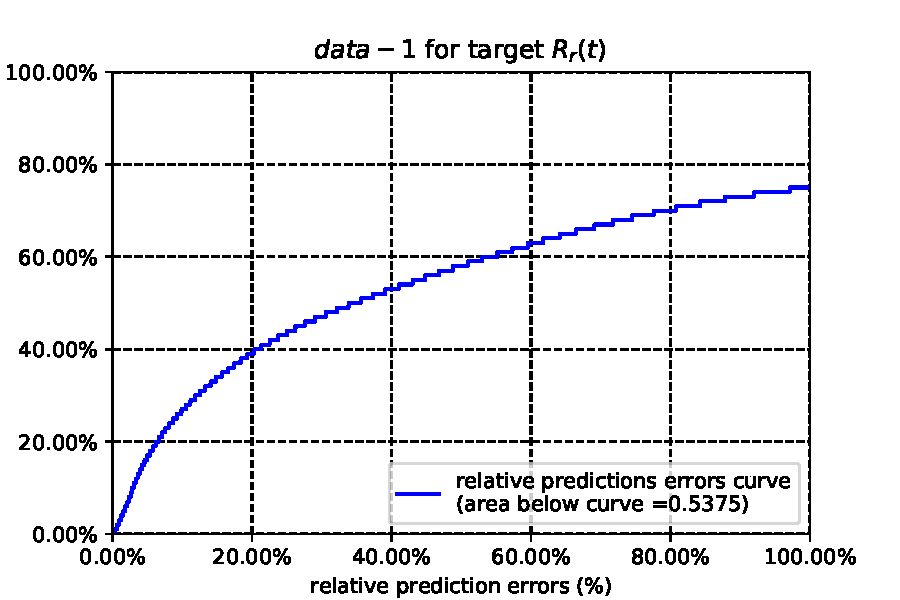
\includegraphics[width=0.3\textwidth]{fig4/data-1-task-1-7030-lstm.pdf}
		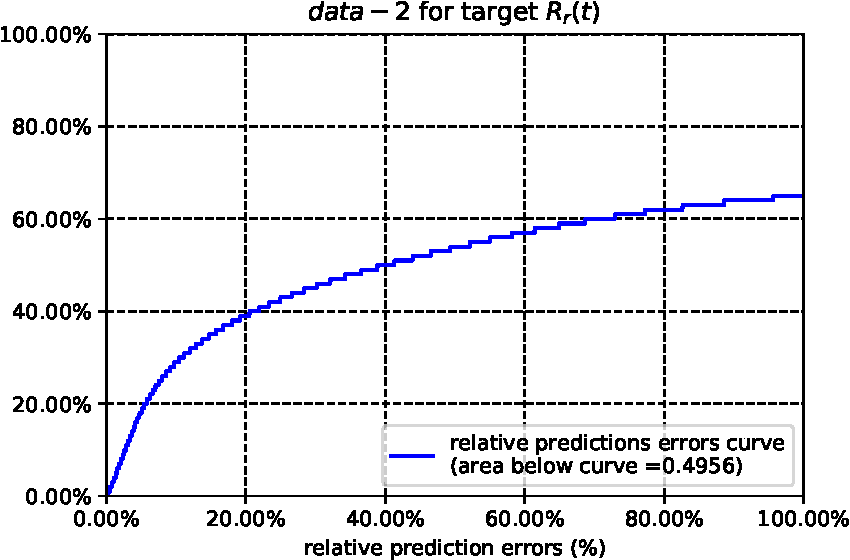
\includegraphics[width=0.3\textwidth]{fig4/data-2-task-1-7030-lstm.pdf}
	\end{figure*} 
	\begin{figure*} 
		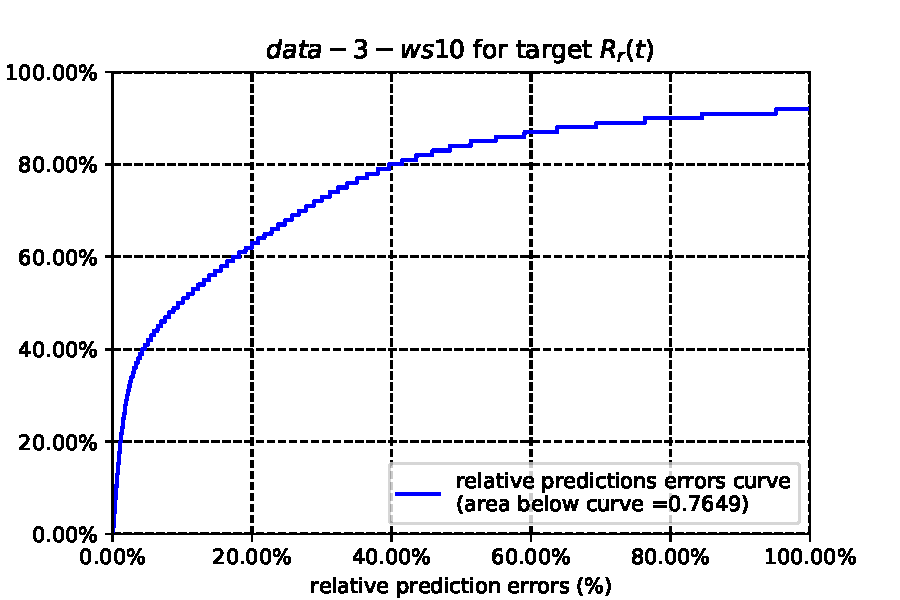
\includegraphics[width=0.3\textwidth]{fig4/data-3-ws10-task-1-7030-lstm.pdf}
		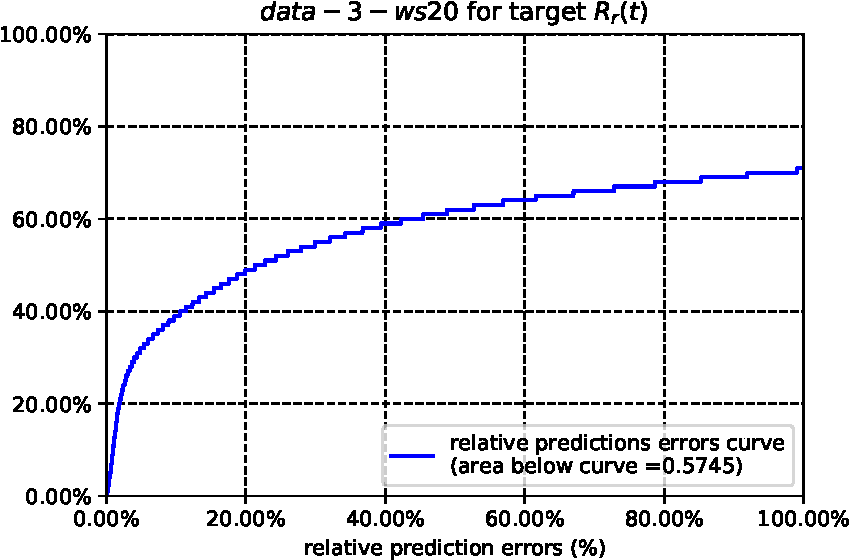
\includegraphics[width=0.3\textwidth]{fig4/data-3-ws20-task-1-7030-lstm.pdf}
		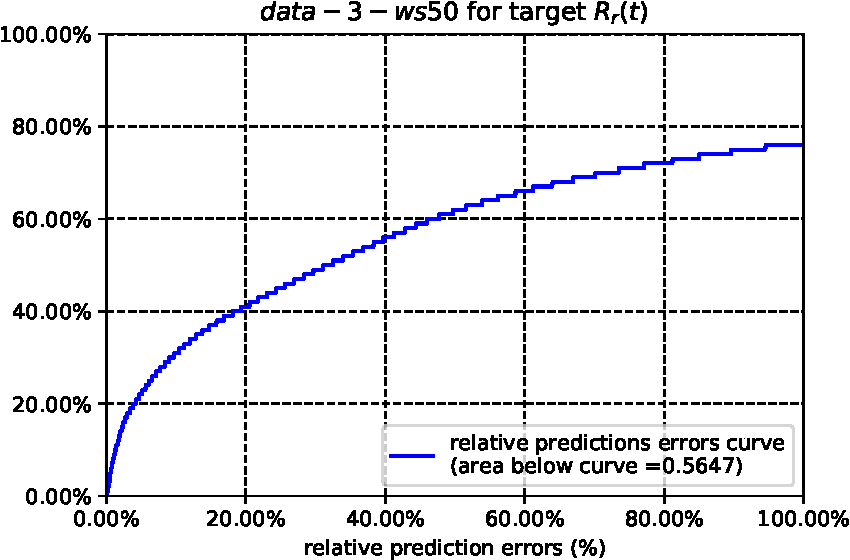
\includegraphics[width=0.3\textwidth]{fig4/data-3-ws50-task-1-7030-lstm.pdf}
		%\vspace{-20pt}  
		\caption{Relative prediction errors for $R_r(t)$ of LSTM models with vector input.}
		\label{fig:lstm-task1-vector}
		%\vspace{-10pt}  
	\end{figure*}
	\begin{figure*} 	
	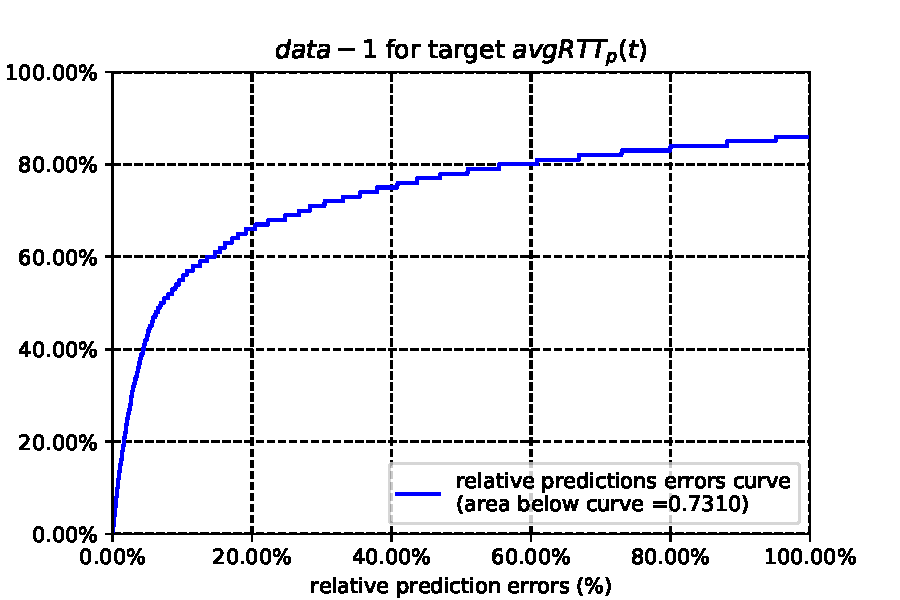
\includegraphics[width=0.3\textwidth]{fig4/data-1-task-3-7030-lstm.pdf}
	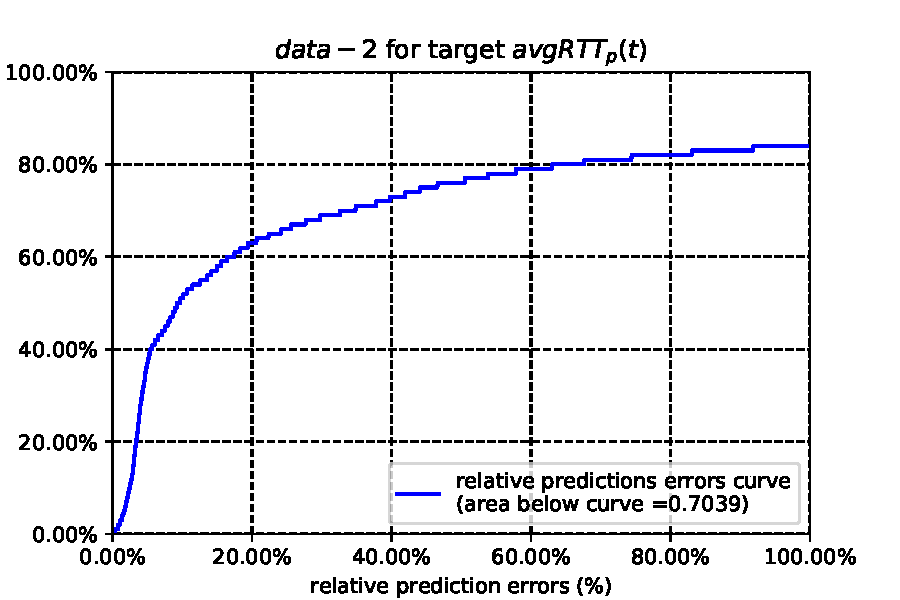
\includegraphics[width=0.3\textwidth]{fig4/data-2-task-3-7030-lstm.pdf}
	\end{figure*} 
	\begin{figure*} 	
	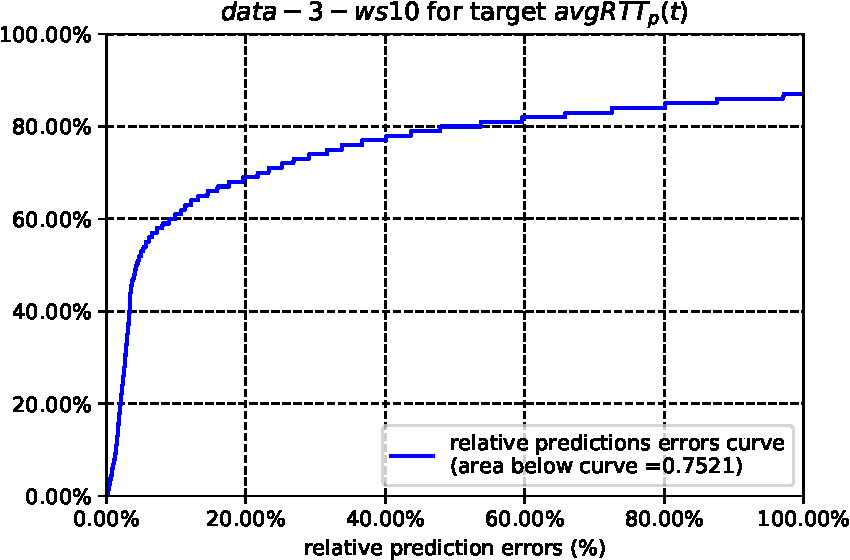
\includegraphics[width=0.3\textwidth]{fig4/data-3-ws10-task-3-7030-lstm.pdf}
	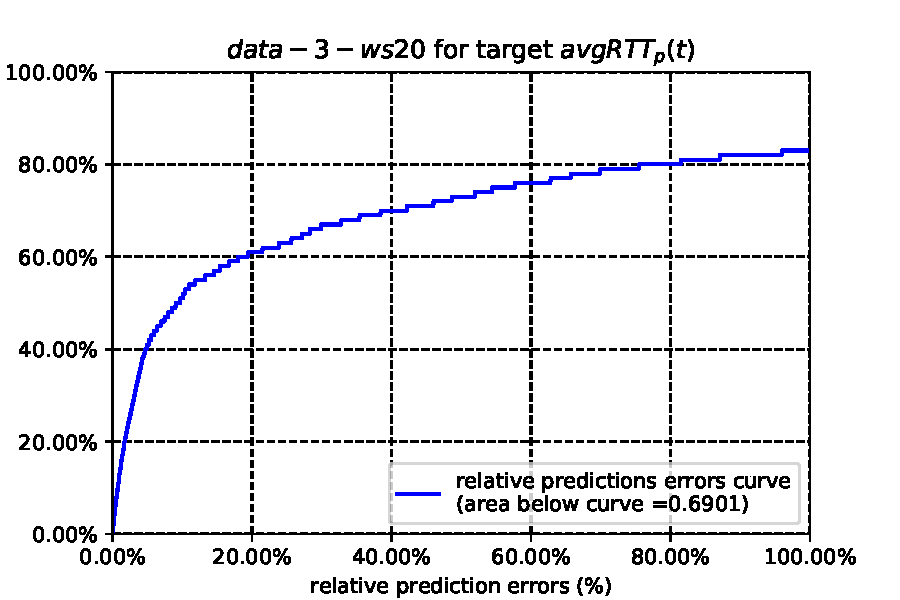
\includegraphics[width=0.3\textwidth]{fig4/data-3-ws20-task-3-7030-lstm.pdf}
	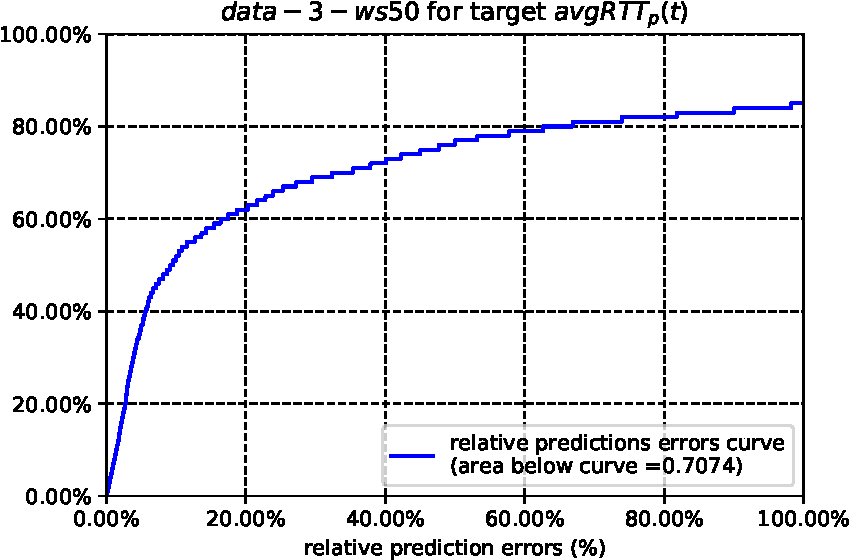
\includegraphics[width=0.3\textwidth]{fig4/data-3-ws50-task-3-7030-lstm.pdf}
	%\vspace{-20pt}  
	\caption{Relative prediction errors for  $avgRTT_P(t)$ of LSTM models with vector input.}
	\label{fig:lstm-task3-vector}
	%\vspace{-10pt}  
	\end{figure*}
	\begin{table}[t]
		\centering
		\begin{tabular}{lcc}
			\toprule
			{Target} &{$R_r(t)$}&{$avgRTT_p(t)$} \\
			\midrule
			\textit{data-1}& 0.5374 & 0.7310 \\
			\textit{data-2}& 0.4956& 0.7039     \\
			\textit{data-3-ws10}& 0.7649 & 0.7521 \\
			\textit{data-3-ws20}& 0.6513& 0.6901    \\
			\textit{data-3-ws50}& 0.5647& 0.7074  \\
			\bottomrule	
		\end{tabular}
		\caption{ Experiment results ($ABC$) of LSTM models with vector input. }
		\label{tab:lstm-vector}
	\end{table}
	
	In general, the results consist with our previous observation that $R_r(t)$ has more temporal locality while $avgRTT_p(t)$ seems to have less or no temporal locality.
	
	More specifically, for target $R_r(t)$, LSTM model outperforms random forest model in all five data processing manners with a maximum $ABC=0.7649$. And when fed with vector input, the LSTM has a significant lift in performance than LSTM with scalar input, which shows that high quality features can be beneficial to not only classic shadow models like random forest, but also \textit{deep} models like LSTM model.
	
	However, when it comes to target $avgRTT_p(t)$, although LSTM models do have better performance when fed with vector input rather than scalar input, their $ABC$s are still smaller than those of random forest. We believe it is because there is less temporal locality with reference to $avgRTT_p(t)$. The more data we observed before, the better we can predict $avgRTT_p(t)$ in the future. Thus LSTM model cannot maximize its ability in predicting temporal patterns.
	\section{Conclusions}
	TODO
	
	\begin{acks}
		TODO
	\end{acks}
	
	
	
	\bibliographystyle{ACM-Reference-Format}
	\bibliography{bibliography} 
	
\end{document}
=======
\documentclass[sigconf]{acmart}

\usepackage{booktabs} % For formal tables
\usepackage{url}
\newcommand{\kai}[1]{{\bf \color{blue} [[Shukai says ``#1'']]}}
\newcommand{\heng}[1]{{\bf \color{cyan} [[Yuheng says ``#1'']]}}
\newcommand{\hao}[1]{{\bf \color{red} [[Hao says ``#1'']]}}
\newcommand{\hui}[1]{{\bf \color{purple} [[Zhenghui says ``#1'']]}}
% Copyright
%\setcopyright{none}
%\setcopyright{acmcopyright}
%\setcopyright{acmlicensed}
\setcopyright{rightsretained}
%\setcopyright{usgov}
%\setcopyright{usgovmixed}
%\setcopyright{cagov}
%\setcopyright{cagovmixed}


% DOI
%\acmDOI{10.475/123_4}

% ISBN
%\acmISBN{123-4567-24-567/08/06}

%Conference
\acmConference[CNW]{SJTU Computer Network Workshop}{December 2017}{Shanghai, China} 
\acmYear{2017}
\copyrightyear{2017}


%\acmArticle{4}
%\acmPrice{15.00}

% These commands are optional
%\acmBooktitle{Transactions of the ACM Woodstock conference}
%\editor{Jennifer B. Sartor}
%\editor{Theo D'Hondt}
%\editor{Wolfgang De Meuter}
